\chapter{Catálogo de Segurança}
\label{chap:proposta}

Neste Capítulo, é apresentada uma primeira versão do Catálogo de Segurança. Dado o volume de aspectos associados à Segurança, procurou-se focar nos tópicos mais relevantes, tendo como base a literatura. Dessa forma, o autor está ciente de que o Catalogo de Segurança não acorda todo e qualquer aspecto associado à Segurança. Mas, a intenção de demonstrar que, um catálogo construído para especificar RNFs, utilizando uma notação adequada, mesmo que em alto nível de abstração, pode colaborar no entendimento das necessidades inerentes aos aspectos não-funcionais de um software, comumente colocados em segundo plano, ou apenas especificados em documentos, em linguagem natural. Esses documentos, como a Especificação Suplementar \cite{sommerville1997requirements}, carecem de uma notação que permita especificar os RNFs com toda a complexidade envolvida, ou seja, partindo de um alto nível de abstração, mas permitindo acordar operacionalizações, as quais de fato tornarão aquele RNF algo implementável, tratável a nível de código. Para a equipe de desenvolvedores, ter especificadas as operacionalizações, pode promover soluções concretas para viabilizar a implementação de aspectos considerados abstratos. Para atingir esse objetivo, o Catálogo de Segurança foi especificado utilizando a notação do NFR \textit{Framework}, já comentada em capítulos anteriores. Essa notação propõe a elaboração de um grafo de interdependências entre os RNFs. Adicionalmente, deixa evidente as principais correlações entre esses RNFs, seus impactos e suas operacionalizações. Conforme justificado no Capítulo \ref{chap:introducao}, dada a relevância do RNF Segurança, têm-se que esse Catálogo de Segurança foca seus esforços na especificação desse RNF.

Para tornar mais compreensível o Catálogo de Segurança, optou-se por apresentá-lo, inicialmente, em dois níveis de abstração. Neste sentido, a seção \ref{sub:primeiroNivel} apresenta o primeiro nível de abstração. Nesse nível, são acordadas as metas flexíveis (representando os RNFs), seus impactos e suas operacionalizações. Utilizou-se a notação do NFR \textit{Framework}, com a elaboração de um grafo, SIG (\textit{Softgoal Interdependence Graph}). Na seção \ref{sub:segundoNivel}, é apresentado um mapeamento, procurando correlacionar as metas flexíveis e as camadas do Padrão Arquitetural MVC. Um terceiro nível de abstração também é mapeado e descritro no Capítulo \ref{chap:resultadosObtidos}, pois para alcançá-lo foi necessário realizar a aplicação do Catálogo de Segurança em cenários. Sendo este, o terceiro nível de abstração entre as operacionalizações e as camadas do Padrão Arquitetural MVC, devido ao fato de envolver aspectos em um nível mais baixo de abstração (implementando de fato as operacionalizações nas camadas \textit{Model-View-Controller}).

\section{O Catálogo de Segurança}

Essa primeira versão do Catálogo de Segurança procura promover, aos especialistas, uma maior compreensão quanto às diferentes necessidades se tratando de Segurança. O Catálogo de Segurança acorda os principais conceitos associados à Segurança, tomando como base o levantamento bibliográfico realizado nessa pesquisa.

Conforme colocado anteriormente, neste capítulo o Catálogo de Segurança será apresentado em dois níveis de abstração. O primeiro nível, descrito na seção \ref{sub:primeiroNivel}, procura apresentar as metas flexíveis - ou RNFs - associadas à Segurança. O grafo especifica ainda, as correlações e os impactos entre essas metas flexíveis bem como, as operacionalizações (no nível mais baixo do grafo). O segundo nível é apresentado na seção \ref{sub:segundoNivel}, como um mapeamento entre as metas flexíveis e as camadas do Padrão Arquitetural MVC.

\subsection{Primeiro Nível de Abstração}
\label{sub:primeiroNivel}

O primeiro nível de abstração apresenta as metas flexíveis mais genéricas de Segurança de software, apoiando-se, principalmente, na definição de Chung. Essa definição se baseia em Confidencialidade, Integridade e Disponibilidade. Adicionalmente, essa abstração também se apoia na definição de Segurança da Informação apresentada na ISO 27001. 

\begin{citacao}
	"Segurança da informação: preservação da \textbf{confidencialidade}, \textbf{integridade} e \textbf{disponibilidade} da informação; adicionalmente, outras propriedades, tais como \textbf{autenticidade}, \textbf{responsabilidade}, não repúdio e \textbf{confiabilidade}, podem também estar envolvidas." \cite[p. 2]{documentation2005information}
\end{citacao}


As metas flexíveis foram definidas de acordo com sua relação com Segurança. Observa-se que foram acrescentados, à notação do SIG, alguns valores representados como referências. A intenção é permitir a rastreabilidade de cada aspecto representado no grafo com sua respectiva fonte ou referência teórica. Esse rastreamento permite ao leitor: (i) ter a comprovação de que a especificação do catálogo foi de fato apoiada na literatura, e (ii) aprofundar seus conhecimentos e, caso assim o desejar, consultar as referências para maior esclarecimento sobre cada especificação sugerida no Catálogo de Segurança. A Tabela \ref{indicesDeReferencia} apresenta os identificadores para a rastreabilidade da referência teórica de uma meta flexível no SIG da Figura \ref{DetalhamentoPrimeiroNivel}. 

\pagebreak

\begin{table}[h!]
	\centering
	\caption{Índices de rastreabilidade.}
	\label{indicesDeReferencia}
	\begin{tabular}{@{}cc@{}}
		\toprule
		\textbf{Identificador} & \textbf{Referência} \\ \midrule
		{[}1{]} & \cite{chung2012non} \\ 
		{[}2{]} & \cite{benitti2015taxonomia} \\
		{[}3{]} & \cite{documentation2005information} \\
		{[}4{]} & \cite{affleck2012supporting} \\
		{[}5{]} & \cite{buschmann1996system}
		\\ \bottomrule
	\end{tabular}
\end{table} 


\begin{figure}[h!]
	\centering
	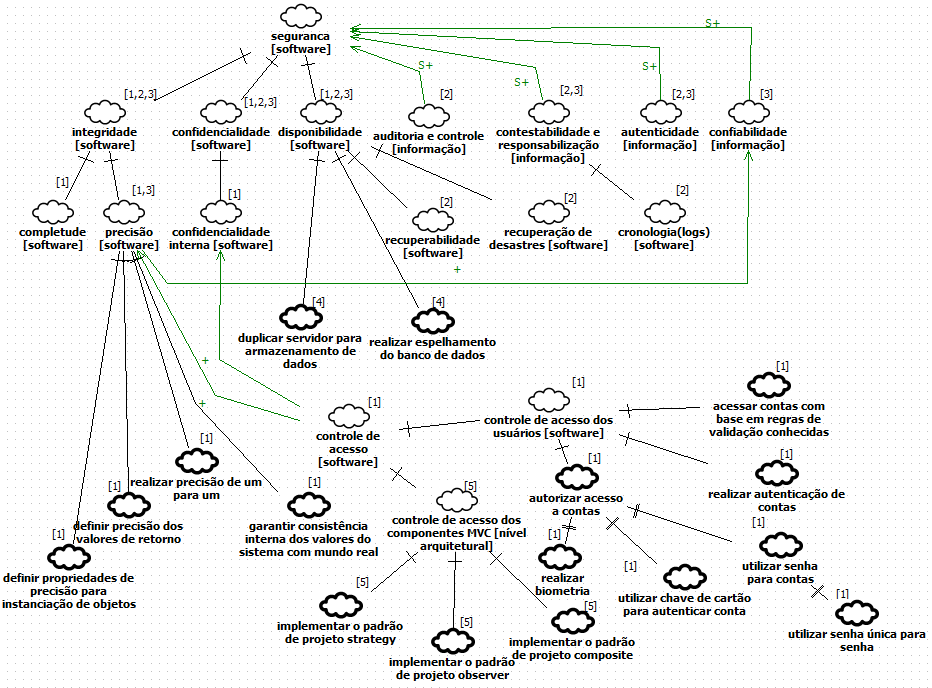
\includegraphics[keepaspectratio=true,scale=0.7]{figuras/CatalogoDeSeguranca.PNG}
	\caption{Catálogo de Segurança.}
	\label{DetalhamentoPrimeiroNivel}
\end{figure}


As definições das metas flexíveis e operacionalizações são: 

\begin{itemize}
	
	\item \textbf{integridade:} proteção contra qualquer tipo de atualização e/ou adulteração não autorizada. Definida na seção \ref{sec:seguranca};
	
	\begin{itemize}
		
		\item \textbf{precisão:} pode ser entendida como qualquer atributo semântico que fundamenta uma informação. Definida na seção \ref{sec:seguranca};
		
		\begin{itemize}
			
			\item \textbf{\textit{definir propriedades de precisão para instanciação de objetos:}} parantir que objetos sejam instanciados da maneira correta. Definida na seção \ref{sec:seguranca};
			
			\item \textbf{\textit{definir precisão dos valores de retorno:}} garantir que os valores retornados pelas operações possuam a precisão pré-estabelecida. Definida na seção \ref{sec:seguranca};
			
			\item \textbf{\textit{realizar precisão de um para um:}} garantir que um único objeto esteja ligado a uma única entidade do domínio. Definida na seção \ref{sec:seguranca};
			
			\item \textbf{\textit{garantir consistência interna dos valores do sistema com mundo real:}} garantir que os valores do mundo real sejam correspondentes aos valores do sistema. Definida na seção \ref{sec:seguranca};
			
			\item \textbf{controle de acesso:} nível mais genérico para autorização de acesso definido por \cite{chung2012non}, trata-se das especificações de controle de acesso do software; 
			
			\begin{itemize}
				
				\item \textbf{controle de acesso dos usuários:} controle de acesso de usuários no software \cite{chung2012non}. Para ser satisfeita, depende de um conjunto de operacionalizações: \textbf{\textit{autorizar acesso a contas}}, \textbf{\textit{acessar contas com base em regras de validação conhecidas}} e \textbf{\textit{realizar autenticação de contas}};
				
				\item \textbf{controle de acesso dos componentes MVC:} trata-se das restrições arquiteturais impostas pelo padrão arquitetural MVC para que as relações internas entre os componentes sejam realizadas \cite{buschmann1996system}. Para que isso ocorra, devem ser implementados três \textit{design patterns}, que são abstraídos no catálogo de Segurança como operacionalizações, sendo elas: (i) \textbf{\textit{implementar o padrão de projeto strategy}}, (ii) \textbf{\textit{implementar o padrão de projeto observer}} e (iii) \textbf{\textit{implementar o padrão de projeto composite}};
				
			\end{itemize}
						
		\end{itemize}
		
		\item \textbf{completude:} garantia que o RNF esteja o mais completo possível. Definida na seção \ref{sec:seguranca};
	\end{itemize}
	
	\item \textbf{confidencialidade:} proteção da informação para evitar que as informações armazenadas ou transmitidas não sejam vistas ou interpretadas por terceiros, sendo somente o usuário principal e o destinatário. Definida na seção \ref{sec:seguranca};
	
	\begin{itemize}
		
		\item \textbf{confidencialidade interna:} proteção da informação que o acesso deve ser evitado por um público externo. Definida na seção \ref{sec:seguranca};
		
	\end{itemize}
	 
	 \item \textbf{disponibilidade:} proteção contra a interrupção do serviço, no momento em que o usuário estiver utilizando a aplicação. Definida na seção \ref{sec:seguranca};
	 
	 \begin{itemize}
	 		
	 		\item \textbf{recuperabilidade:} intervalo de tempo que o software deverá estar disponível após uma falha \cite{benitti2015taxonomia};
	 	
	 		\item \textbf{recuperação de desastres:} políticas e procedimentos aplicados na recuperação de ``desastres`` induzidos no software por usuário ou softwares de terceiros \cite{benitti2015taxonomia};
	 		
	 		\item \textbf{\textit{duplicar servidor para armazenamento de dados:}} promove menor chance de tempo onde ocorra a inatividade dos dados. Com a utilização de dois ou mais servidores em funcionamento, a disponibilidade dos dados do software é maior \cite{date2004introduccao}\cite{affleck2012supporting};   
	 		
	 		\item \textbf{\textit{realizar espelhamento do banco de dados:}} compreende-se como duas cópias de um único banco de dados que geralmente reside em máquinas diferentes \cite{date2004introduccao}\cite{affleck2012supporting}; 
	 		
	 \end{itemize}
 
 	\item \textbf{auditoria e controle:} especificação dos aspectos que devem ser contemplados para proporcionar a auditoria e o controle \cite{benitti2015taxonomia}; 
 	
 	\item  \textbf{contestabilidade e responsabilização:} capacidade do software em quantificar as ações e os eventos, com intuito de comprovar sua ocorrência \cite{benitti2015taxonomia}; 
 	
 	\begin{itemize}
 		
 		\item \textbf{cronologia(logs):} registro de alterações no software \cite{benitti2015taxonomia};
 		
 	\end{itemize}
 	
 	\item \textbf{autenticidade:} capacidade do software em identificar que um objeto ou recurso é o que ele realmente declara ser \cite{benitti2015taxonomia}, e
 	
 	\item \textbf{confiabilidade:} capacidade do software em realizar e manter seu funcionamento quando submetido em circunstâncias de rotina \cite{benitti2015taxonomia}. 
 	
\end{itemize}

\subsection{Segundo Nível de Abstração}
\label{sub:segundoNivel}

O segundo nível de abstração procura correlacionar as metas flexíveis mais genéricas e as camadas do Padrão Arquitetural MVC. As Tabelas \ref{mapeamento1} e \ref{mapeamento2} apresentam esse mapeamento, considerando diferentes níveis de satisfação para cada meta flexível.


\begin{table}[h!]
	\centering
	\caption{Mapeamento das metas flexíveis com as camadas do MVC - Parte 1.}
	\label{mapeamento1}
	\tiny
	\begin{tabular}{@{}cccp{5cm}cc@{}}
		\toprule
		\multicolumn{1}{l}{\textbf{id}} & \multicolumn{1}{l}{\textbf{Meta flexível}} & \multicolumn{1}{l}{\textbf{\begin{tabular}[c]{@{}l@{}}Nível de\\ satisfação\end{tabular}}} & \multicolumn{1}{l}{\textbf{Descrição}} & \multicolumn{1}{l}{\textbf{Referência}} & \multicolumn{1}{l}{\textbf{Camada}} \\ \midrule
		1 & \begin{tabular}[c]{@{}c@{}}“precisão\\ {[}software{]}”\end{tabular} & \begin{tabular}[c]{@{}c@{}}Suficientemente\\ Satisfeita\end{tabular} & Garante que um ou mais objetos estejam ligados a uma única entidade do domínio. Além disso, impacta diretamente a \textit{Model} pois é a camada que representa os aspectos do domínio da aplicação.
		
		
		- Atributo de precisão: precisão de um para um. & \begin{tabular}[c]{@{}c@{}}\cite{chung2012non}\\ \cite{buschmann1996system}\end{tabular} & \textit{model} \\
		
		\rowcolor[HTML]{C0C0C0} 2 & \begin{tabular}[c]{@{}c@{}}“precisão\\ {[}software{]}”\end{tabular} & \begin{tabular}[c]{@{}c@{}}Suficientemente\\ Satisfeita\end{tabular} & Garante que os objetos sejam instanciados da maneira correta dentro da \textit{model}.
		
		- Atributo de precisão: Propriedade da precisão. & \begin{tabular}[c]{@{}c@{}}\cite{chung2012non}\\ \cite{buschmann1996system}\end{tabular} & \textit{Model} \\
		
		3 & \begin{tabular}[c]{@{}c@{}}“autenticidade\\ {[}informação{]}”\end{tabular} & \begin{tabular}[c]{@{}c@{}}Satisfeita\\ Suficientemente\end{tabular} & A utilização de \textit{triggers} em banco de dados promove a autenticidade e a verificação da integridade do dado. Além disso, pode ser utilizada para realização de auditoria em tabelas. &  &  \\
		\cellcolor[HTML]{C0C0C0}4 & \cellcolor[HTML]{C0C0C0}\begin{tabular}[c]{@{}c@{}}“integridade\\ {[}software{]}”\end{tabular} & \cellcolor[HTML]{C0C0C0}\begin{tabular}[c]{@{}c@{}}Satisfeita\\ Suficientemente\end{tabular} & \cellcolor[HTML]{FFFFFF} &  &  \\
		5 & \begin{tabular}[c]{@{}c@{}}“auditoria e\\  controle\\ {[}informação{]}”\end{tabular} & \begin{tabular}[c]{@{}c@{}}Satisfeita\\ Suficientemente\end{tabular} & \multicolumn{1}{l}{} & \multirow{-3}{*}{\cite{date2004introduccao}} & \multirow{-3}{*}{\begin{tabular}[c]{@{}c@{}}Banco \\ de Dados\end{tabular}} \\
		
		\rowcolor[HTML]{C0C0C0} 
		\multicolumn{1}{l}{\cellcolor[HTML]{C0C0C0}6} & \begin{tabular}[c]{@{}c@{}}“controle\\  de acesso usuário\\ {[}software{]}”\end{tabular} & \begin{tabular}[c]{@{}c@{}}Parcialmente\\ Satisfeita\end{tabular} & O método de autenticação dos dados retorna a instância do usuário, quando a senha está correta. Esse aspecto é implementado diretamente na \textit{Controller}. Entretanto, possui clara relação com a \textit{View} e com a base de dados. Considera-se “Parcialmente Satisfeita”, pois há dependência com a operacionalização “Autorizar Acesso a Contas", a qual contribui para a satisfação dessa meta flexível “controle de acesso {[}software{]}”. & \cite{fuentes2014ruby} & \textit{Controller} \\
		
		\multicolumn{1}{l}{7} & \begin{tabular}[c]{@{}c@{}}“confiabilidade\\ {[}informação{]}”\end{tabular} & \begin{tabular}[c]{@{}c@{}}Suficientemente\\ Satisfeita\end{tabular} & Garante que o conjunto de dados a serem armazenados na base de dados estejam relativamente fidedignos. Usa-se “relativamente”, pois não há como garantir algo pleno, se tratando de critérios tão abstratos. Nesse caso, “relativamente” sugere que seja o mais fidedigno/confiável possível”. & \cite{fuentes2014ruby} & \textit{View} \\ 
		
		\rowcolor[HTML]{C0C0C0} 
		8 & \begin{tabular}[c]{@{}c@{}}“controle de \\ acesso dos \\ componentes \\ MVC\\ {[}nível arquitetural{]}”\end{tabular} & \begin{tabular}[c]{@{}c@{}}Parcialmente\\ Satisfeita\end{tabular} & Garante que os componentes da \textit{View}, os quais dependem de outros componentes que se encontram em outras camadas do modelo MVC, reconheçam a necessidade de atualizar as telas, adequando-as às demandas encaminhadas via \textit{Controller} (por exemplo) e em compatibilidade com os dados especificados na \textit{Model}. Considera-se “parcialmente satisfeita”, pois há dependência com a implementação do padrão de projeto estrutural \textit{Composite}. A implementação é sugerida como operacionalização que contribue para satisfação dessa meta flexível, “controle de acesso dos componentes MVC {[}nível arquitetural{]}.” & \begin{tabular}[c]{@{}c@{}}\cite{baptistella2011abordando} \\ \cite{buschmann1996system}\end{tabular} & \textit{View} \\
		
		\bottomrule
	\end{tabular}
\end{table}

\begin{table}[p]
	\centering
	\caption{Mapeamento das metas flexíveis com as camadas do MVC - Parte 2.}
	\label{mapeamento2}
	\tiny
	\begin{tabular}{@{}cccp{5cm}cc@{}}
		\hline
		\multicolumn{1}{l}{\textbf{id}} & \multicolumn{1}{l}{\textbf{Meta flexível}} & \multicolumn{1}{l}{\textbf{\begin{tabular}[c]{@{}l@{}}Nível de\\ satisfação\end{tabular}}} & \multicolumn{1}{l}{\textbf{Descrição}} & \multicolumn{1}{l}{\textbf{Referência}} & \multicolumn{1}{l}{\textbf{Camada}} \\ \hline
		\rowcolor[HTML]{C0C0C0} 
		8 & \begin{tabular}[c]{@{}c@{}}“controle de \\ acesso dos \\ componentes \\ MVC\\ {[}nível arquitetural{]}”\end{tabular} & \begin{tabular}[c]{@{}c@{}}Parcialmente\\ Satisfeita\end{tabular} & Garante que os componentes da \textit{View}, os quais dependem de outros componentes que se encontram em outras camadas do modelo MVC, reconheçam a necessidade de atualizar as telas, adequando-as às demandas encaminhadas via \textit{Controller} (por exemplo) e em compatibilidade com os dados especificados na \textit{Model}. Considera-se “Parcialmente Satisfeita”, pois há dependência com a implementação do padrão de projeto estrutural \textit{Composite}. A implementação é sugerida como operacionalização que contribue para satisfação dessa meta flexível, “controle de acesso dos componentes MVC {[}nível arquitetural{]}.” & \begin{tabular}[c]{@{}c@{}}\cite{baptistella2011abordando} \\ \cite{buschmann1996system}\end{tabular} & \textit{View} \\
		9 & \begin{tabular}[c]{@{}c@{}}“controle de\\ acesso dos \\ componentes\\ MVC\\ {[}nível arquitetural{]}”\end{tabular} & \begin{tabular}[c]{@{}c@{}}Parcialmente\\ Satisfeita\end{tabular} & Garante que a \textit{Model} esteja menos acoplada em relação à \textit{View} e à \textit{Controller}, viabilizando essa relação através de boas práticas da Engenharia de Software. Uma dessas práticas é sugerida como operacionalização na Figura \ref{DetalhamentoPrimeiroNivel}, apoiando-se no uso de Padrões de Projeto. Considera-se parcialmente satisfeita, pois há dependência com a implementação do padrão de projeto comportamental \textit{Observer}, por exemplo. Essa implementação é sugerida como uma operacionalização possível em atendimento a essa demanda e contribui para a satisfação dessa meta flexível, “controle de acesso dos componentes MVC{[}nível arquitetural{]}”. & \begin{tabular}[c]{@{}c@{}}\cite{baptistella2011abordando} \\ \cite{buschmann1996system}\end{tabular} & \textit{Model} \\
		\rowcolor[HTML]{C0C0C0} 
		10 & \begin{tabular}[c]{@{}c@{}}“controle de\\ acesso dos \\ componentes\\ MVC\\ {[}nível arquitetural{]}”\end{tabular} & \begin{tabular}[c]{@{}c@{}}Parcialmente\\ Satisfeita\end{tabular} & Garante menor acoplamento entre as camadas MVC. Sugere-se que tal aspecto seja apoiado no uso de Padrões de Projeto. Portanto, acredita-se que o padrão de projeto \textit{Strategy}, implementado na \textit{Controller}, permita menor acoplamento entre \textit{View} e \textit{Model}, sendo, de fato, responsabilidade da \textit{Controller} intermediar essa relação utilizando decisões estratégicas. Vale ressaltar que, com o uso desse padrão de projeto decisões podem ser tomadas em tempo de execução, alterando o comportamento do software em função das demandas conhecidas dinamicamente. Dessa forma, a tendência é de maior cumprimento de boas práticas já acordadas no padrão arquitetural MVC. Considera-se parcialmente satisfeita, pois há dependência com a implementação do padrão de projeto comportamental \textit{Strategy}, por exemplo. Essa implementação é sugerida como uma operacionalização possível em atendimento a essa demanda, e contribui para a satisfação dessa meta flexível, “controle de acesso dos componentes MVC{[}nível arquitetural{]}”. & \begin{tabular}[c]{@{}c@{}}\cite{baptistella2011abordando} \\ \cite{buschmann1996system}\end{tabular} & \textit{Controller} \\ \hline
	\end{tabular}
\end{table}

\pagebreak
\pagebreak

\section*{Resumo do Capítulo}

Neste capítulo, foi apresentada uma primeira versão do Catálogo de Segurança proposto nessa pesquisa. Adicionalmente, foram apontados os principais impactos e as contribuições das informações do Catálogo de Segurança em relação às camadas do Padrão Arquitetural MVC. Ressalta-se que, o Catálogo foi especificado apoiando-se na literatura, conforme pode ser observado considerando a rastreabilidade, apresentada na seção \ref{sub:primeiroNivel} evidenciando o primeiro nível de abstração, onde foi descrito as metas flexíveis associadas à Segurança. o Catálogo de Segurança especificou as correlações e os impactos entre as metas flexíveis bem como, as operacionalizações. O segundo nível de abstração foi apresentado na seção \ref{sub:segundoNivel}, demonstrando o mapeamento entre as metas flexiveis e as camadas do Padrão Arquitetural.

Por fim, cabe mencionar que, o Catálogo de Segurança ainda possui mais um nível de abstração, o qual será demonstrado no Capítulo \ref{chap:resultadosObtidos}, pois só foi possível mapear a correlação entre as operacionalizações e as camadas MVC, 
com a aplicação em cenários, permitindo apresentar como os critérios de qualidade podem ser suficientemente tratados e satisfeitos a nível de código.
